\documentclass[twoside,11pt]{article}

% Any additional packages needed should be included after jmlr2e.
% Note that jmlr2e.sty includes epsfig, amssymb, natbib and graphicx,
% and defines many common macros, such as 'proof' and 'example'.
%
% It also sets the bibliographystyle to plainnat; for more information on
% natbib citation styles, see the natbib documentation, a copy of which
% is archived at http://www.jmlr.org/format/natbib.pdf

\usepackage{jmlr2e}
\usepackage[ruled,vlined]{algorithm2e}

% Definitions of handy macros can go here

\newcommand{\dataset}{{\cal D}}
\newcommand{\fracpartial}[2]{\frac{\partial #1}{\partial  #2}}

% Heading arguments are {volume}{year}{pages}{date submitted}{date published}{paper id}{author-full-names}

%\jmlrheading{1}{2000}{1-48}{4/00}{10/00}{meila00a}{Marina Meil\u{a} and Michael I. Jordan}

% Short headings should be running head and authors last names

\ShortHeadings{Alternating Transfer Learning}{Fornia}
\firstpageno{1}

\begin{document}

%\title{Machine Learnable Image Compression Using Convolutional Autoencoders}
\title{Using Alternating Transfer Learning to Create Multi-Purpose Layers
in Deep Convolutional Neural Networks}

\author{\name R. Paul Fornia \email paulfornia@gmail.com \\
       \addr Department of Computer Science\\
       Johns Hopkins University\\
       Baltimore, MD, USA
       %\AND
       %\name bob...\\
       }

%\editor{Kevin Murphy and Bernhard Sch{\"o}lkopf}

\maketitle

\begin{abstract}%   <- trailing '%' for backward compatibility of .sty file
With transfer learning, image classification Convolutional Neural Network (CNN)
 layers can be initialized by 
parameters of a different pre-trained network (e.g.,
an autoencoder (AE), or a CNN from a different
classification task).
These layers are then typically fine-tuned to better 
fit the new task, in effect producing a new, distinct
network.

I extend this idea by producing early layers of parameters that 
actually fit into
a high performing AE and a high performing CNN classifier simultaneously. 

First, I test the effectiveness of creating these layers simply from an AE or a CNN,
and then applying them in a fixed, non-trainable way to the opposite context
(AE trained on classification layers,
and vice-versa). 
This step is essentially traditional transfer learning, but on a network 
designed to function as an AE and classifier simultaneously.
Next, I propose a methodology called Alternating Transfer Learning (ATL)
that transfers the layers
back and forth between the two contexts. Finally, I test the application of 
ATL to images from an entirely different domain.

Of these four methods, only (in-domain) ATL performs highly,
and nearly matches performance of the more traditional AE and CNN trained end-to-end.
The other three tests perform respectably, and may be sufficient for some appications,
but fall short of the performance of the traditional baselines.

I discuss potential applications, including
generating lossy compressed images on which inference can be
performed without the need to first decompress the image. Further refinement of 
the ideas proposed in this paper are needed before such applications are practical
or valuable.

%practical image compression framework that performs well as both 
%a) a traditional file compression and b) a feature set for which image 
%classification can be performed with high accuracy. If successful, this would 
%allow for highly accurate image classification to be applied directly to compressed 
%images and may speed up training and fitting of image classifiers. I 
%begin with a simplified version of the Compressive AE (CAE), 
%which has already demonstrated 
%promise as an image compression system, but which has not been tested directly 
%in classification. I also propose a \emph{context-specialized} image compression, in
%which an AE (such as a CAE) is used to initialize a classification problem, the 
%labels are used to fine-tune the Deep Convolutional Neural Network (DNN)
% (as has been discussed in the classification
%literature), a middle layer is quantized and taken as the compression, and new 
%layers are trained on the compression (using the original image as the output) 
%to turn it back into an effective AE.
\end{abstract}

\begin{keywords}
    Autoencoder, Compression, Convolutional Neural Network, Image Classification,
    Transfer Learning
\end{keywords}




\section{Background and Literature}

\subsection{Transfer Learning}

Transfer learning is the practice of using existing parameters from a solved problem
to initialize (or outright replace) portions of parameters in a new context.
While transferring can be done with many machine learning techniques, \citet{oquab2014learning}
 provides the basic framework for CNN transfer learning.
Like this paper (and unlike some transfer learning techniques) they perform a 
``fixed'' transfer, in effect finding ``Mid-Level'' layers
to represent images that can be used in two distinct networks. Unlike this paper, the two
networks are both trying to achieve classification tasks, and the parameters are simply trained
on one task and transferred to another. There is no attempt to simultaneous optimize these 
parameters to work well on both tasks. Also unlike this paper, since neither task is an
AE, the data representation is simply a set of features, and there is not necessarily any
ability to reconstruct the images from this representation. It is therefore not a lossy
compression in the same way that this paper's representation is.

\citet{yosinski2014transferable} provide a similar, but more theoretical look at 
CNN transfer learning. They characterize layers near the input as general-purpose filters,
and layers near the target variable as specialized, and they imagine an approximate boundary where
this shift occurs. Similar to this paper, they seek to transfer ``general purpose'' layers,
but like \citet{oquab2014learning}, they do not discuss the application to compression that
could be achieved if enough layers can be made general.

\subsection{Image Classification in Practice and Motivation}
The use of images in data pipelines is extremely common across industries and 
domains. Many of these applications include both image file compression and 
image classification steps. But many modern pipelines approach these as two 
separate problems – often first ingesting and compressing
images for storage, and then when needed for classification 
(training or fitting), they must be uncompressed back into a lossy version, 
similar to their original human-readable form.

 For instance, Facebook has published details of both compression and their 
facial recognition algorithm, and there is no indication that the two systems 
are integrated \citep{collet2016zstandard, taigman2014deepface}.

\subsection{Existing Efforts Toward Machine Learnable Compression}

As several authors have noted, 
there would be considerable value in being able to perform machine learning 
tasks directly on the compressed images. \citet{needell2017} has written a classification 
algorithm that can be performed on any general binary file structure (including 
state-of-the art image compression methods), but this approach has not yet shown
 competitive classification performance. 

Conversely, \citet{fu2016} showed strong 
classification performance, but on cosine distance, which is not a competitive 
compression algorithm. The same can be said for any approach that performs 
embeddings or feature extraction, which can be viewed as a form of compression 
designed specifically for one ML task.

I seek a balanced approach that perform as well at compression,
and for which the compressed images 
can be classified without the need for decompression, with out-of-sample
 classification accuracy near that of an analogous CNN trained end-to-end.

I begin with the AE, which was originally 
devised as a compression algorithm, and has also inspired many elements of 
deep learning, which is the backbone of virtually all competitive image 
classification algorithms today.
AEs have many practical applications outside of compression, including 
pretraining deep neural networks, feature extraction, 
and image de-noising \citep{baldi2012autoencoders}. While some authors have claimed that AEs do 
not have practical value as compression algorithms,
%\footnote{
%Multiple practical guides make this claim. For instance, \citet{huben2018_tds_ae} states ``autoencoders will 
%do a poor job for [out-of-sample] image compression... JPEG will do vastly better.''
%}
recent work by 
\citet{theis2017} and \cite{cheng2018deep} propose a compressive, convolution autoencoder (CAE) that 
has shown great promise as an effective, practical image compression method, 
competitive with the JPEG file format.


\subsection{Contributions}

This paper lays a foundation by proposing
a high level NN architecture, where an AE and a classification CNN
share an identical set of input layers. This ``left'' set of layers\footnote{I 
will refer to NNs as running 
left-to-right, moving from the input data to the labels}
can be interpreted as a machine learnable compression, since the output of these
layers can be both decompressed and classified separately. 

In order to actually train this architecture, I try four methods of increasing complexity.
The first two are essentially just transfer learning with fixed parameters, first
transferring AE to a classifier, and then vice-versa.

The third method, which I call Alternating Transfer Learning (ATL), is the most novel 
and academically interesting contribution of this paper.
It is also successful in its goal strictly speaking: to train layers 
that are simultaneously used in two effective NNs. Unlike other transfer learning,
these parameters are trained by both tasks, not just one,
thus I hope to push the limits of general layers as described by \cite{yosinski2014transferable}.
With ATL, one can create an image compression
that can be decompressed efficiently, and upon which we can perform inference in a 
classification application. 

However, because ATL requires supervised labels, its practical usefulness is still limited,
since it does not allow classification to be \emph{trained} on an already-built compression scheme.
In other words, full images are still needed at the time of training, as the training 
impacts the compression method. 

With this in mind, I present a fourth method, which is to apply the results of ATL to brand-new
domain. This would provide more obvious practical value, but performance results 
from experiments are mixed.

%There are similarities to existing literature. For example, some papers have used
%unsupervised techniques to produce feature sets for supervised learning \citep{bengio2006pretrain}.






\section{Methodology} \label{fixed}

For all techniques proposed in this paper, the intended compression framework has
three high-level components to its architecture, which are
 illustrated in Figure \ref{fig:three_stages}:
\begin{enumerate}
    \item Compression layers, which are the ``left half'' of either an AE or CNN. 
    \item Decompression layers, which are the ``right half'' of an AE. 
    \item Classification layers, which can be interpreted as either the right half of
     an end-to-end CNN classifier, or as the entire classifier trained on extracted (compressed) features. This portion can easily and quickly be retrained for each new classification problem.
\end{enumerate}

All methodologies tried in this paper produce these three components.

\begin{figure}[h]
  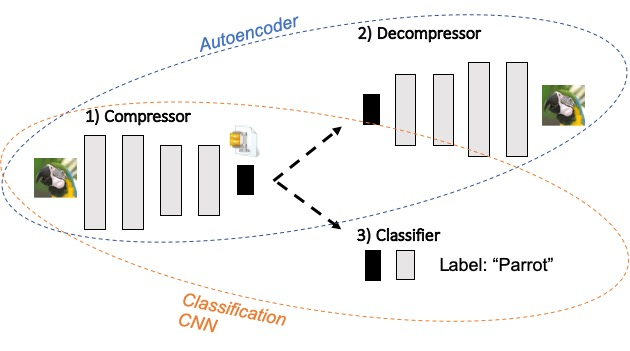
\includegraphics[width=\linewidth]{figures/three_stages.jpg}
  \caption{The three-stage machine learnable compression framework contains a compressor, 
  a decompressor, and a classifier. Stages 1 and 2 together make an AE, stages 1 and 3 
  together make a classification CNN. This paper considers the sharing of the 
  compressor between both tasks. }
  \label{fig:three_stages}
\end{figure}

\subsection{Classification from AE-driven Compression} \label{general}

For the first methodology, I start with an AE approach in order 
to produce a traditional compression on the image data (components 1 and 2). 
I then take the resulting compressed data (i.e., the bottleneck layer) and attempt 
to perform classification
to predict the categorical labels (component 3).
This process is illustrated in Figure \ref{fig:general}.

\begin{figure}[h]
  \includegraphics[width=\linewidth]{figures/general.jpg}
  \caption{The AE-driven compression framework. Blue layers are trained with image targets (like an AE).
  Green layers are trained with class labels.}
  \label{fig:general}
\end{figure}

\subsection{Decompression from Classifier-driven Compression} \label{special}

Having tested the efficacy of AE layers in a classifier, I similarly transfer layers to an
AE that are constructed in a classification CNN.
I first replicate a high-performing classification CNN from the literature. 
I then select one of the hidden layers, and apply simple
quantization techniques. This hidden layer 
will act as the compressed image. This CNN will make up components 1 and 3.
Then, using the original image as a target, I train a new decompression layer (component 2).  
This is illustrated in Figure \ref{fig:specialized}.

\begin{figure}[h]
  \includegraphics[width=\linewidth]{figures/specialized.jpg}
  \caption{The Classifier-driven compression framework.}
  \label{fig:specialized}
\end{figure}

Since components 1 and 2 are effectively built off standard classification CNNs, 
this model’s efficacy as a classifier has already been shown at length in the 
literature \citep{krizhevsky2012imagenet}. I will reproduce this finding to create a 
baseline performance level. I then test whether 
the decompressor performs similarly to the analogous end-to-end AE.



\subsection{Alternating Transfer Learning} \label{alternate}

In section \ref{results} below, I will show that the performances of the above methods are limited. 
Simply copying the lower layers from one context to another 
does not provide performance comparable to end-to-end training. 
Thus, the compression obtained by an AE
is not an effective feature set for classification, and the lower levels of a classifier 
CNN do provide parameters for a competitive compression technique. 

Having shown that an AE or CNN alone does not produce a good general-purpose compression,
the question still remains on whether any such compression exists. 
The idea presented in this section is simple, and is motivated by 
the standard transfer learning procedure. I continuously transfer the shared
initial layers back-and-forth between different contexts while training until results converge. 

The proposed technique is shown in Algorithm \ref{alg:alternate}.

\begin{algorithm}[H]
\SetAlgoLined
\KwResult{Compression, Decompression, and Classification NN components}
 Initialize model parameters for compression, decompression and classification layers;
 \While{Either Classifier or AE Performance is improving}{
  %\eIf{condition}{
  % instructions1\;
  % instructions2\;
  % }{
  % instructions3\;
  %}
  Train entire AE (compressor and decompressor) for $k_{AE}$ epochs\;

  Train only Classifier layers for $j_{Class}$ epochs, as in Section \ref{fixed}\;

  Measure Classification performance\;

  Train entire Classification CNN (compressor and classifier) for $k_{Class}$ epochs\;

  Train only Decompressor layers for $j_{AE}$ epochs\;

  Measure AE performance\;
 }
 Fine tune only Classifier layers by training a few epochs;

 Fine tune only Decompressor layers by training a few epochs;
 \caption{Alternating Transfer Learning procedure}
 \label{alg:alternate}
\end{algorithm}


\subsection{Extension of ATL training to other domains}

The ATL methodology is interesting and unique, but the application is not immediately obvious.

Greater value would come from machine learnable compression layers if the layers could
be learned in advance of having a classification problem, and then quickly learned without
need for decompressing images. One final approach I test is taking parameters from the ATL 
procedure learned on one domain of images, and then attempted to learn both a classifier
and a decompressor on images from a brand-new domain. While all experiments use unseen images from a test
set, this approach takes it a step further and trains these tasks in a brand new domain,
using images unlike those seen in training. 

This architecture is shown in Figure \ref{fig:ext_atl}.

\begin{figure}[h]
  \includegraphics[width=\linewidth]{figures/ext_atl.jpg}
  \caption{The extension of the Alternating Transfer Learning framework to a new domain.}
  \label{fig:ext_atl}
\end{figure}

As I discuss in the results section, this technique yields mixed results, and tasks from 
one domain are not able to be easily learned from the compressed layers that had been trained
using ATL on a different domain. 










\section{Experiments and Results} \label{results}


\subsection{Datasets}

I use three datasets in this paper:

\begin{enumerate}
\item{MNIST: Handwritten digits 0-9 \citep{lecun2010mnist}}
\item{KMNIST: Examples of ten handwritten Japanese characters \citep{clanuwat2018deep}}
\item{Fashion-MNIST: Images of ten categories of clothing or accessories \citep{xiao2017fashion}}
\end{enumerate}

These datasets are all greyscale, all 28x28 pixels, and all consist of ten classes.
In fact, KMNIST and Fashion-MNIST were created as easy ``drop-in'' replacements for MNIST.
A future direction of research could be to test color images and images of varying sizes.
Using images from different domains can provide a starting point for transferring 
compression representations, even if the structure of the images from the different 
domains is very similar.

\subsection{Performance Metrics}

As all three datasets contain ten well-balanced classes, I simply use accuracy to measure
effectiveness of classification. 

\begin{equation}
Accuracy = \frac{Correct\ Predictions}{Total\ Predictions}
\end{equation}

For the AE, I measure performance by Peak Signal to Noise Ratio (PSNR), 
a conversion of Mean Squared Error (MSE) into the decibel scale, which is a common
performance metric of reconstructing lossy image compressions.

\begin{equation}
PSNR = 10*log_{10}\left(\frac{MAX^2_I}{MSE}\right)
\end{equation}

Where $MAX_I$ is the maximum pixel value, e.g. 255.


\subsection{Architecture}

For this paper, I propose an architecture for experimental purposes.
There is one primary constraint on the architecture design as shown in Figure \ref{fig:three_stages}:
the initial layers of the AE must match initial layers of the classification network.
Here, ``initial layers of the AE'' mean all layers from the input to the bottleneck layer (inclusive).

I do not claim that the proposed architecture is the optimal one for this problem,
however, the architecture is loosely based on existing well performing networks, and so 
results are still strong enough for many practical applications.
Future research could focus on improvements to this architecture.

I begin with the popular but simple LeNet architecture \citep{lecun1998gradient}, 
with a small modification to account for the size of the MNIST data.
I also add dropout layers in the fully connected portion of the graph. 
This powerful addition helps prevent overfitting, and was popularized long
after the publication of LeNet \citep{srivastava2014dropout}.

The LeNet architecture also has another valuable property: a good bottleneck layer.
The last convolutional layer of LeNet contains about half the parameters of the input,
similar to the bottleneck layer in many AE architectures. 

To create the Decompression layers, I simply work backwards from the compression layers of LeNet,
using similar convolutions, and upsample layers in place of maxpool layers.
I also add an additional convolutional layer, which I found to improve AE performance.

Finally, I add a quantization to the bottleneck layer by rounding output values, as is done
by \citet{theis2017}.
The input values of the datasets contain 28x28 pixels of integer values between 1 and 255.
The uncompressed image therefore is represented in $28*28*log2(256) = 6272 = 784$ bytes.
The bottleneck layer contains 16 5x5 filters. 
After rounding the compressed values, outputs were integers between 0 and 15,
allowing compressed images to be stored in just $16*5*5*log2(16) = 1600 = 200$ bytes,
for a data compression ratio of 3.9, or space savings of 74.5\%. 
Another future enhancement to this methodology could be to utilize more advance quantization techniques
such as those described by \citet{hubara2018}.

%%Table of architecture here%%

\begin{table}[h]
  \centering
  \begin{tabular}{|c|c||c|c||c|c|}
    \hline
    %\multicolumn{2}{|c|}{Baseline (50 Epochs of Training)}\\
    %\hline
    \multicolumn{2}{|c||}{1) Compressor} & 
    \multicolumn{2}{|c||}{2) Decompressor} & 
    \multicolumn{2}{|c|}{3) Classifier}\\  
    \hline
    Layer Type & Output & Layer Type & Output & Layer Type & Output \\  
    \hline
    Input & 1x28x28 & Compressed Input & 16x5x5 & Compressed Input & 16x5x5\\  
    \hline
    6 5x5 Conv Filters & 6x24x24 & Upscale & 16x10x10 & Flatten & 400\\  
    \hline
    Padding & 6x28x28 & Padding & 16x14x14 & Full Layer & 120\\  
    \hline
    Max Pooling 2x2 & 6x14x14 & 16 3x3 Convolutions & 16x12x12 & 50\% Dropout & 120\\  
    \hline
    16 5x5 Conv Filters & 16x10x10 & Upscale & 16x24x24 & Full Layer & 84\\  
    \hline
    Max Pooling 2x2 & 16x5x5 & Padding & 16x28x28 & 50\% Dropout & 84\\  
    \hline
     &  & 6 3x3 Convolutions & 6x26x26 & Full Layer & 10\\  
    \hline
     &  & Padding & 6x30x30 &  & \\  
    \hline
     &  & 1 3x3 Convolution & 1x28x28 &  & \\  
    \hline

  \end{tabular}
  \caption{The architecture used for these experiments, broken into the three components
    described in Section \ref{fixed}}
  \label{table:base}
\end{table}



\subsection{Baseline AE and Classifier}

While the architecture above is based on a classifier with good performance,
the architecture (especially the AE) is not necessarily state-of-the art. 
So, in order to measure performance, I first run 50 epochs of both the full AE and Classification CNN,
both with randomly initialized parameters, allowing for the full network to be trained,
just as a traditional deep neural network would be. 
I measure performance on the test dataset as training progresses,
and find that improvement has largely leveled off by the 50th epoch, and does not appear to overfit.
This provides a good best-case-scenario benchmark for performance of the AE and Classifier. 

%%%Table of Baseline findings%%%%
%\begin{table}
%  \centering
%  \includegraphics[]{figures/table_baseline.jpg}
%  \caption{Baseline performance metrics of the full AE and Classification CNN. 
%   Measured on an out-of-sample test dataset after 50 epochs of training.}
%  \label{table:base}
%\end{table}

\begin{table}[h]
  \centering
  \begin{tabular}{|c||c|c|}
    \hline
    \multicolumn{3}{|c|}{Baseline (50 Epochs of Training)}\\
    \hline
    Dataset & Classification Accuracy & Decompression PSNR \\
    \hline
    MNIST & 98.6\% & 22.8\\
    \hline
    KMNIST & 89.9\% & 17.0\\
    \hline
    Fashion & 85.7\% & 18.2\\
    \hline
  \end{tabular}
  \caption{Baseline performance metrics of the full AE and Classification CNN. 
   Measured on an out-of-sample test dataset after 50 epochs of training.}
  \label{table:base}
\end{table}

\subsection{AE-Driven Compression Experiment} \label{expAE}

As described in section \ref{general}, I start with the baseline AE.
Using the lower layers, I compress all the images. This in effect ``freezes'' the 
lower layer parameters, and does not allow them to be fine-tuned. 
I then train only the classifier layers on the compressed image.

%%%Insert Findings here%%%

\begin{table}[h]
  \centering
  \begin{tabular}{|c||c|c|}
    \hline
    \multicolumn{3}{|c|}{Classification trained on AE-Driven compression}\\
    \hline
    Dataset & Baseline Accuracy & Accuracy on Compressed Data \\
    \hline
    MNIST & 98.6\% & 91.7\%\\
    \hline
    KMNIST & 89.9\% & 70.7\%\\
    \hline
    Fashion & 85.7\% & 79.8\%\\
    \hline
  \end{tabular}
  \caption{Performance metrics of the General Compression: 
   Accuracy on an out-of-sample test dataset after 50 epochs of training a classifier on
   data compressed by the AE.}
  \label{table:general}
\end{table}

I find that, for all three datasets, the classification accuracy on the compressed images
is reasonably high (possibly good enough for some applications), but significantly 
less than that of the baseline.


\subsection{Classifier-Driven Compression Experiment} \label{expClass}

As described in section \ref{special}, I start with the full classification CNN.
As above, I use the lower layers of this network to compress the image, then I train
only the decompressor layers on the compressed images, with the original images
as the target values.

%%Insert table%%

\begin{table}[h]
  \centering
  \begin{tabular}{|c||c|c|}
    \hline
    \multicolumn{3}{|c|}{AE trained on Classifier-Driven compression}\\
    \hline
    Dataset & Baseline PSNR & PSNR on Compressed Data \\
    \hline
    MNIST & 21.8 & 19.9\\
    \hline
    KMNIST & 17.0 & 15.4\\
    \hline
    Fashion & 18.2 & 17.8\\
    \hline
  \end{tabular}
  \caption{Performance metrics of the Specialized Compression: 
   PSNR on an out-of-sample test dataset after 50 epochs of training an AE on
   data compressed by the Classification CNN.}
  \label{table:special}
\end{table}

Just as with the classification based on the AE-driven compression attempt, 
I find an AE with some value, but with 
significantly worse performance than the AE that is trained from the original images.

\subsection{Alternating Transfer Learning Experiment}

Next, I test the idea described in Section \ref{alternate} by implementing Algorithm \ref{alg:alternate}.
For each of the three datasets separately, I train the AE layers, then the Classification layers
(which include shared layers with the AE, which have now been initialized), then train the AE again,
and so on. I define an ``epoch set'' as one round of all four types of training as described in 
Algorithm \ref{alg:alternate}. For this experiment, I set $k_AE = k_class = j_AE = j_class = 1$, 
meaning each epoch set contains a total of four epochs (each of differing levels of complexity).
Further research is needed to optimized these hyperparameters.

For all three datasets, I perform 25 epoch sets. With a total of 100 epochs, this is roughly
similar run time to the above experiments, which require 50 full epochs (e.g., end-to-end AE
to train the network from scratch), and 50 epochs on the smaller network component 
(e.g., classification on the fixed, compressed image set).

%%%% Insert Findings %%%%

\begin{table}[h]
  \centering
  \begin{tabular}{|c||c|c|c|c|}
    \hline
    \multicolumn{5}{|c|}{Alternating Transfer Learning}\\
    \hline
    Dataset & Baseline PSNR  & PSNR from ATL & Baseline Accuracy & Accuracy from ATL \\   \hline
    MNIST & 21.8 & 22.8 & 98.6\% & 97.2\% \\   \hline
    KMNIST & 17.0 & 17.6 & 89.9\% & 85.5\% \\   \hline
    Fashion & 18.1 & 18.5 & 85.6\% & 85.2\% \\   \hline  

  \end{tabular}
  \caption{Performance metrics of the Alternating Transfer Learning:
   PSNR on an out-of-sample test dataset after 50 epochs of training an AE on
   data compressed by the Classification CNN.}
  \label{table:alternate}
\end{table}

As shown in table \ref{table:alternate}, this method outperforms the other methods proposed so far.
For all six tests (classification and AE for three datasets), the Alternating Transfer Learning 
approach significantly outperforms the simple fixed transfers described above. 

Classification accuracy of these approaches is slightly below that of the traditional 
end-to-end CNN approach, however, PSNR on the decompressed images actually exceeds that
of the traditional full AE, and performance trends over the epoch sets suggest further room
for improvement. 

\subsection{Extension to Other Domains}

Above, I find that the ATL network performs well on new images of the same domain (e.g., 
handwritten digits). The final experiment tests whether the compression layers trained
by the ATL methodology can used to learn AEs or classifiers on images and tasks in a 
different domain (e.g., Japanese character recognition).

Similar to the experiments in sections \ref{expAE} and \ref{expClass}, I use compressor
layers from an existing network -- in this case from ATL. I use them to produce compressed
image representations (effectively freezing the compressor parameters) of data
from a new domain, and then train 
new classifier and decompressor layers for the new tasks. 

With three datasets, I can conduct 6 pairs of tests: ATL trained on MNIST extended to
KMNIST, ATL trained on MNIST extended to Fashion, etc.. For each of these pairs of tests, 
I perform both AE and classification. After training the ATL as described above, 
I train the classifier and decompressor layers for 50 epochs each.

%%%% Table of results %%%%%

\begin{table}[h]
  \centering
  \begin{tabular}{|c||c|c|c|c|c|c|}
    \hline
    \multicolumn{7}{|c|}{Out-of-Domain Performance}\\
    \hline
    ATL Domain & \multicolumn{2}{|c|}{From MNIST} & 
      \multicolumn{2}{|c|}{From MNIST}& \multicolumn{2}{|c|}{From MNIST}\\
    \hline
    New Domain & KMNIST & Fashion & MNIST & Fashion & MNIST & KMNIST\\  \hline    
    Accuracy & 69.7\% & 78.8\% & 75.0\% & 77.7\% & 91.3\% & 62.3\%\\  \hline
    PSNR & 16.8 & 18.6& 22.9& 19.2 & 21.3& 16.4\\  \hline
  \end{tabular}
  \caption{Performance metrics of ATL compression extended to new domains:
   Accuracy/PSNR on an out-of-sample test dataset after 50 epochs of 
   training an Classifier/Decompressor on
   data compressed by ATL.}
  \label{table:domain}
\end{table}


Performance from each of these tests is shown in table \ref{table:domain}. Results are mixed.

First, let's consider classification, where we see varying results. For example, the MNIST 
classifier is able to achieve 91\% accuracy trained only on the compressed image, where
the compressor was created by the ATL process using the Fashion dataset. This is lower than 
the baseline CNN, but comparable to the compressor trained using an AE on other MNIST data,
and may be high enough for some applications. This is impressive considering that the compression
algorithm had not only never seen any of the test images, but had never even seen an image
that resembled anything like a hand-written digit. Yet the features, which were forced to be 
balanced to accommodate both and AE and Classifier (from a different domain), proved 
general-purpose enough to provide some classification accuracy to a new domain.

These results were not entirely consistent. For example, the KMNIST classification problem
(using ATL from the Fashion dataset) only achieved 62\% accuracy -- far better than random,
but worse than the in-domain methods, and likely not high enough for practical
applications.

Fortunately, AE shows more consistent and positive results.
The out-of-domain PSNR beats out the baseline
AE, and performs almost as well as the ATL decompression. 
One possible explanation for this finding is that
domain does not matter as much for image decompression as it does for classification. In all
domains, the AE is simply trying to reconstruct image pixels, and this appears to work even 
when images from one domain look dramatically different from those of another.

One other observation from this test is that, unlike the other experiments, performance does \emph{not}
seem to converge after 50 epochs. Further exploration is warranted to determine a)
how much more these models can improve, and b) how many more epochs are needed to achieve
this higher performance.
%% Insert chart here of non-convergence??








\section{Discussion}

\subsection{Practical Implications}

To my knowledge, this paper is the first to provide a framework for training two 
separate neural network architectures that share sets of parameters. 
While this is an interesting academic accomplishment, the networks that I trained 
in this paper via the ATL methodology fall short of having obvious practical applications.

The original motivation for this work was to find a compression method that could act as
the input to a classification CNN. If one considers the two tasks in classification,
training and inference, I succeeded at this goal in one sense and fell short in another. 
The ATL is a functioning compression algorithm for which inference can be performed directly
on the compressed version of the images, at greatly reduced speed. However, since labels
were used in creating the ATL, the training step itself was not performed on the compressed 
images, but rather on a combination of compressed and uncompressed images. 

This is unfortunate, since the practical implications for training on compressed images 
is more obvious than the implications for inference on compressed images. Training on 
compressed images would allow new widely applicable, general compression techniques to 
be used for general purpose image storage, with the knowledge that new problems could be
applied at a later time with decompressing. By contrast, if the classification task is
already known at the time the compression is developed (which it must be for ATL), 
then it is easy enough to simply perform inference at the time of
image compression, since the class label itself is trivially small to store. 

There is one possible scenario in which findings of this paper could have a direct, practical
application: those in which
fast training is more important than accuracy. In this case, the AE-driven compression
method can be used, and a classifier can be trained directly on the compressed image very quickly.
The results here show that this method gets an accuracy lower than a traditional 
classification CNN, but still far above random, and likely high enough for some applications.

\subsection{Run-Time}

Run-time of training and inference for the above methods is critical to the practicality
of these methods. In a highly informal test\footnote{I average the run-time of ten epochs,
and make some calculations based on assumptions around overhead and additivity of steps
(e.g., time to backpropagate equals time to train less time for inference).
All experiments are run with standard Jupyter notebooks using PyTorch and Python 3
on a Model 2017 Macbook Air (1.8 GHz Intel Core i5) with no other processes running.},
I estimate compute time for each component, shown in table \ref{table:runtime}.

%%% table here %%%

\begin{table}[h]
  \centering
  \begin{tabular}{|c|c|}
    \hline
    Component/Direction & Time (Sec/Epoch) \\   \hline \hline
    Compress/Forward & 10 \\ \hline  
    Compress/Back & 16 \\ \hline
    Decompress/Forward & 44 \\ \hline
    Decompress/Back & 62 \\ \hline
    Classify/Forward & 1 \\ \hline
    Classify/Back & 7 \\ \hline 
  \end{tabular}
  \caption{Approximate Run Time of network components for feed forward and back propagation
    steps. Inference (i.e., compression) uses only feed forward steps, while training
    uses both forward and backward steps. One epoch contains 60,000 images broken into 
    batches of 512.}
  \label{table:runtime}
\end{table}

These estimates have several important implications. First, compression is fast,
but decompression is slow. This is likely due to the extra layer used in the 
decompressor architecture, and further work should be done to explore ways to speed up this step.
Furthermore, this time should be more rigorously compared to other image compression techniques.

Second, \emph{training} the decompressor is much slower than training the
compressor.
This imposes limitations on the potential for training domain specific decompressors on 
existing compressors, since it is not much additional effort to train the entire AE.

Finally, by contrast, classifier training is faster than compressor training.
This suggests that training a classifier on already compressed images is far faster 
than training an end-to-end classification CNN on a per epoch basis. This suggests real 
value in being able generate machine learnable compressions.  

\subsection{PyTorch Implementation}

I attempted versions of this project both in TensorFlow (via python) and PyTorch, 
and settled on PyTorch.
The methods in this paper have two unique implementation elements.
This first is to have an architecture
with two targets, two loss functions, etc.. Surprisingly, this was easy in both tools, by
simply having code for components 2) and 3) both reference the last layer from component 1).
Then, with some care, you can train 2) (which backpropagates to component 1)) without 
affecting component 3), and then train 3) without affecting 2).

The slightly trickier aspect was ``freezing'' the parameters in 1) altogether, 
which is a critical step for this approach, and which differentiates this from traditional
transfer learning. This can be done manually in any tool by simply performing inference
to get the outputs of the bottle-neck layer, then feeding this into a brand-new NN as input,
and finally transferring the parameters back into the original architecture.

However, with PyTorch, this can be done simply with the detach() function.
This effectively freezes the value, and breaks the mapping of the backpropagation gradient, 
and preserves all prior layer parameters.

All training in this paper uses 60,000 28x28 8-bit integer-valued pixels.
An epoch uses all 60,000 images, broken into batches of 512. Performance metrics are
run against 10,000 test images that are not included in training.

\subsection{Next Steps}

There are at least three obvious paths forward for future research.

First, the ideas of ATL must be expanded to more practical training methodologies. 
More experimentation should be done to find other architectures with shared layers.
Using the three components proposed here, there are many possible 
ways to train this architecture, even if the architecture's components themselves are fixed.
One potential next step is to expand ATL beyond two domains. ATL accomplishes two tasks:
AE and Classification for one domain. But this could be easily expanded to more than one domain. 
Just from the data used in this study, ATL could be performed alternating between six different 
tasks: Decompressing MNIST, Classifying MNIST, Decompressing KMNIST, etc..
As it was performed in this paper, ATL trained on one domain did not extend to another.
But I would hypothesize that ATL trained on several domains may generalize to new ones better.  

Second, steps should be taken to be used on more realistic images. The methods described
in this paper could easy be extended to color images. Also, techniques could be explored that
are intended to handle images of differing sizes. A simple solution to this is resizing
so that all input images have the same dimensions,
but some architectures have been designed to handle different sized images
without the need for resizing \citep{Iandola2016ExploringTD}.
This would support the idea in the above paragraph, since handling images of differing sizes
would greatly increase the number of label classification sets available.


Finally, ideas should be incorporated from the AE literature to improve PSNR and the 
data compression rate. 
As a proof of concept, I used an AE that fit nicely with the classification network.
But state-of-the-art compressive AEs can achieve much higher PSNR with better data
compression ratios. For example, \citet{theis2017} achieves a PSNR of over 40 with 
substantially better compression ratios than what I use here. 
One challenge will be to find early layer architectures that balance the benefits
of both state-of-the-art
AEs, and state-of-the-art classifiers.  



%  blah blah sample citation ~\citep{pearl:88}.  Whether in their guise as 
%random fields), \emph{probabilistic graphical models} have a number 
%of uncertainty...\\

%{\noindent \em Remainder omitted in this sample. See http://www.jmlr.org/papers/ for full paper.}

% Acknowledgements should go at the end, before appendices and references

%\acks{We would like to acknowledge support for this project
%from the National Science Foundation (NSF grant IIS-9988642)
%and the Multidisciplinary Research Program of the Department
%of Defense (MURI N00014-00-1-0637). }

% Manual newpage inserted to improve layout of sample file - not
% needed in general before appendices/bibliography.

%\newpage

%\appendix
%\section*{Appendix A.}
%\label{app:theorem}

% Note: in this sample, the section number is hard-coded in. Following
% proper LaTeX conventions, it should properly be coded as a reference:

%In this appendix we prove the following theorem from
%Section~\ref{sec:textree-generalization}:

%\noindent
%{\bf Theorem} {\it Let $u,v,w$ be discrete variables such that $v, w$ do
%not co-occur with $u$ (i.e., $u\neq0\;\Rightarrow \;v=w=0$ in a given
%dataset $\dataset$). Let $N_{v0},N_{w0}$ be the number of data points for
%which $v=0, w=0$ respectively, and let $I_{uv},I_{uw}$ be the
%respective empirical mutual information values based on the sample
%$\dataset$. Then
%\[
%	N_{v0} \;>\; N_{w0}\;\;\Rightarrow\;\;I_{uv} \;\leq\;I_{uw}
%\]
%with equality only if $u$ is identically 0.} \hfill\BlackBox

%\noindent
%{\bf Proof}. We use the notation:
%\[
%P_v(i) \;=\;\frac{N_v^i}{N},\;\;\;i \neq 0;\;\;\;
%P_{v0}\;\equiv\;P_v(0)\; = \;1 - \sum_{i\neq 0}P_v(i).
%\]
%These values represent the (empirical) probabilities of $v$
%taking value $i\neq 0$ and 0 respectively.  Entropies will be denoted
%by $H$. We aim to show that $\fracpartial{I_{uv}}{P_{v0}} < 0$....\\

{%\noindent \em Remainder omitted in this sample. See http://www.jmlr.org/papers/ for full paper.}


\vskip 0.2in
%\bibliographystyle{unsrt}
\bibliography{paper}

\end{document}
